
%(BEGIN_QUESTION)
% Copyright 2011, Tony R. Kuphaldt, released under the Creative Commons Attribution License (v 1.0)
% This means you may do almost anything with this work of mine, so long as you give me proper credit

Mange moderne distribuerte kontrollsystemer (DCS) har også programvare for kommunikasjon med HART-aktiverte instrumenter. Ett eksempel på slik programvare er Emersons {\it AMS}:

$$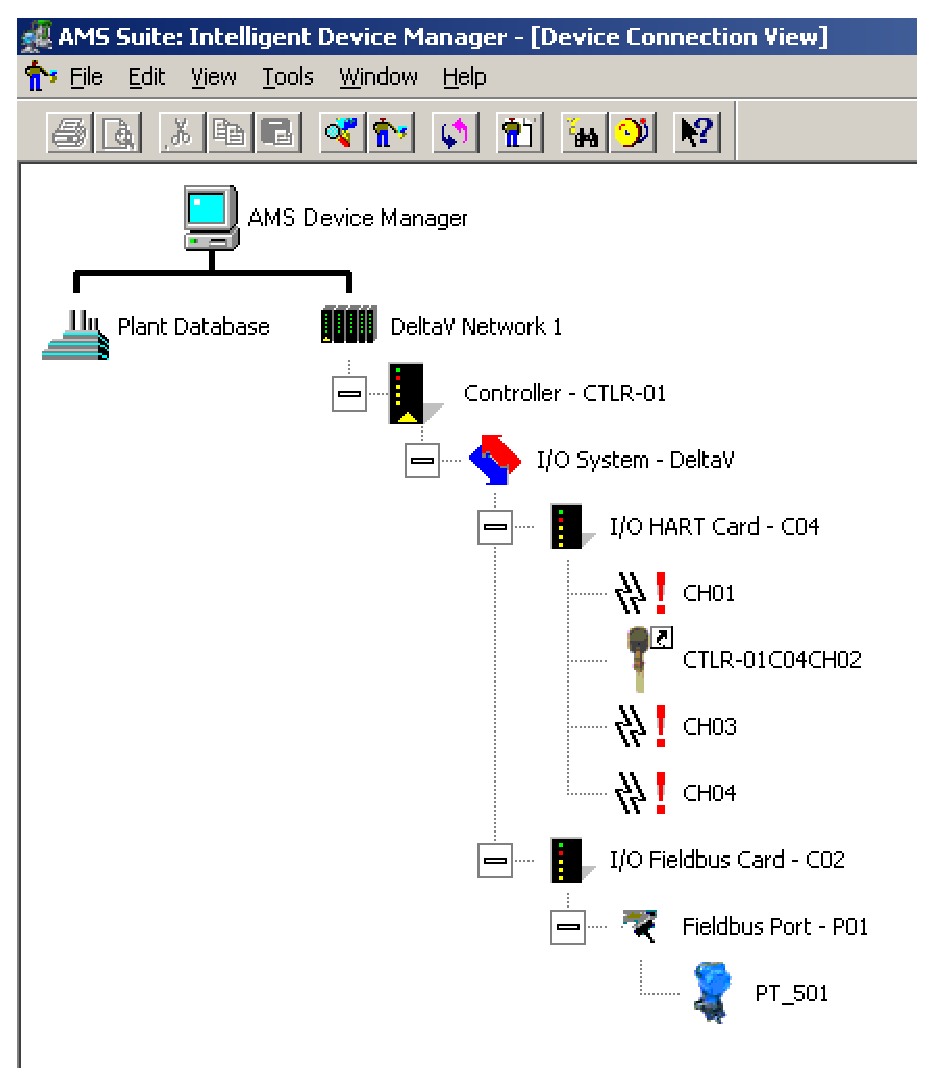
\includegraphics[width=15.5cm]{i00665x01.eps}$$

Hva avslører dette skjermbildet om HART-instrumentene som er koblet til dette Emerson DeltaV-DCS-et? Hvilke fordeler kan oppnås ved at DCS-et kan kommunisere digitalt med feltinstrumenter? Hvilke ulemper ser du med denne metoden for HART-grensesnitt, sammenlignet med en håndholdt HART-kommunikator?

\vskip 20pt \vbox{\hrule \hbox{\strut \vrule{} {\bf Forslag til sokratisk diskusjon} \vrule} \hrule}

\begin{itemize}
\item{} Når DCS-et er aktivert for å "snakke" HART med feltinstrumenter, kan man ikke samtidig bruke en håndholdt HART-kommunikator til å "snakke" med de samme instrumentene. Forklar hvorfor.
\end{itemize}

\underbar{file i00665no}
%(END_QUESTION)





%(BEGIN_ANSWER)

En ulempe er at når du bruker programvare som AMS til å vise og/eller redigere HART-parametere fra kontrollrommet, får du ikke samme verifikasjon av at du har riktig instrument som når du kobler en håndholdt HART-kommunikator direkte til instrumentet.

%(END_ANSWER)





%(BEGIN_NOTES)

Skjermbildet fra Emerson AMS viser ikke bare hvilken kanal hvert HART-instrument er koblet til, men også hvilken instrumenttype det er (hver type med sitt eget grafiske ikon).

%INDEX% DCS, HART-instrumentgrensesnitt
%INDEX% Emerson AMS-programvare

%(END_NOTES)
